\section{Distributed Flow Migration}
\label{sec:fm}

In this section, we present a lightweight, distributed flow migration protocol for \nfactor, designed to circumvent inefficiencies observed for flow migration in exising NFV systems. 

\subsection{Main Idea}

In most existing work \cite{gember2015opennf, rajagopalan2013split}, flow migration is tightly coupled with implementation of the NF software. To migrate flows from a NF, not only large amounts of patch code needs to be added for extracting and transmitting NF states, but also the centralized controller is heavily involved, leading to a scalability issue. Migration of a specific flow has to be initiated by the controller \cite{gember2015opennf}; during the migration process, the controller has to exchange messages with migration source, migration target and the SDN switch. 


We build the flow migration functionalities as message handlers of the actors, and provide flow migration as a basic operation in \nfactor. Flow migration is transparent to implementation of the NF module, eliminating the need of patch code. On the other hand, flow migration is initiated by the actor that processes the flow, and only involves 3 passed of request-response messages in sequence, making the entire process lightweight and scalable. 

Based on the actor model, flow migration can be regarded as a transaction between a source actor and a target actor, where the source actor delivers its entire state and processing tasks to the target actor. Flow migration is successful once the target actor has completely taken over packet processing of the flow. %, when the source actor can safely quit.
 In case of unsuccessful flow migration, the source actor can fallback to regular packet processing and instruct to destroy the target actor.
 

%This is the of NFActor
%framework. There are some problems with existing flow migration
%framework \cite{gember2015opennf, rajagopalan2013split}. First they all use a
%centralized controlelr to monitor the entire flow migration
%process. This is not scalable. The second problem is that the flow migration
%protocol is too complicated to implement. Patch code needs to be added to the
%core processing logic of the NFs. The flow migration protocol needs to exchange
%multiple messages among controller, switches and NF instances. This increases
%the possibility of serious software bugs. The final problem is that the NF can
%not start the flow migration process by itself. It must be started from the
%controller. This stops the NFs from making timely responses to overload signal.

%All the above mentioned problems could be solved using NFActor framework. In
%NFActor framework, the NF packet processing is carried out within the
%execution context of the actor. This additional layer of monitoring gives
%NFActor power to start flow migration from the NFActor runtime. On the other
%hand, the API design forces a clean separation between flow state and NF
%processing logic, making extracting and serializing flow state an easy task.
%NFActor framework also has a built-in message-passing functionality that
%makes flow migration simpler. In this section, we elaborate in detail how flow
%migration works in NFActor framework.

\subsection{Distributed Flow Migration Protocol}

We next present the details of our flow migration procedure. 


\textbf{Initiate Flow Migration.} In \nfactor, flow migration is primarily used to resolve hot spot (overloaded runtimes), or shut down idle runtimes. Each runtime keeps monitoring its CPU and memory usage. If thresholds on resource consumption are exceeded (Sec.~\ref{sec:implementation}), the runtime starts migrating flows to other runtimes with a smaller load. The runtime keeps a local copy of the workload of other runtimes through the view service. Whenever runtime would like to migrate a actor, it selects a target runtime with a smaller workload and notifies the actor about the target runtime% \chuan{discuss more about how to select the target runtimes in a fully distributed fashion.} 
If the controller detects an idle runtime, it will turn the state of the idle runtime into ``\textit{leaving}''. Then the idle runtime starts migrating all its flows to other runtimes before the controller shuts it down. Idle runtime rejects all the migration requests from other actors to keep other actors from migrating to it. %\chuan{if the idle runtime is selected as migration target, would its state return to running? Discuss here.}

To notify a flow to migrate to another runtime (the migration target runtime system), the current runtime sends the ID of the migration target runtime to the actor handling the flow. Then the actor starts migrating the flow by itself, using the flow migration steps described below. %in \cref{sec:dfmp}. 


%\subsection{Distributed Flow Migration Protocol}
%\label{sec:dfmp}

\begin{figure*}[!t]
	\begin{subfigure}[t]{0.30\linewidth}
		\centering
		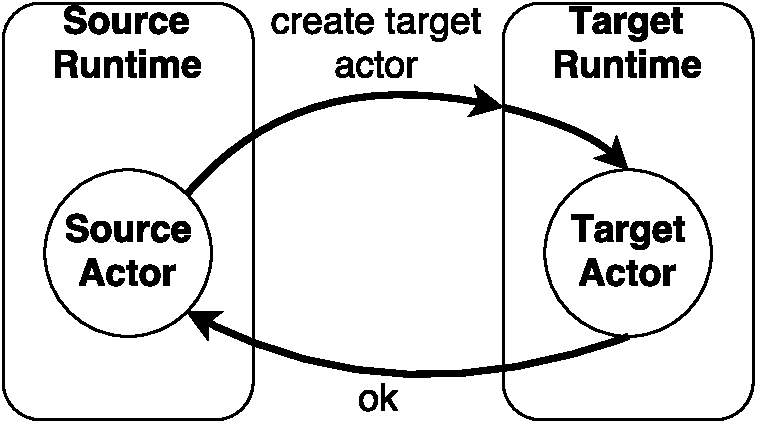
\includegraphics[width=\columnwidth]{figure/NFActor-Flow-Migration-First.pdf}
		\caption{Create target actor}\label{fig:first} \end{subfigure}\hfill
	\begin{subfigure}[t]{0.30\linewidth}
		\centering
		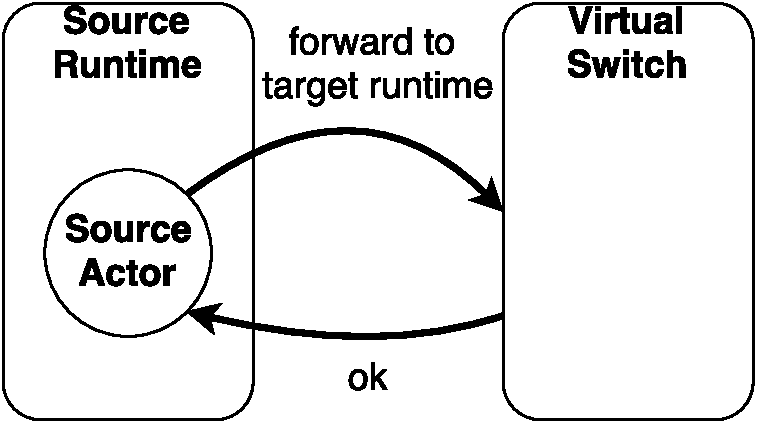
\includegraphics[width=\columnwidth]{figure/NFActor-Flow-Migration-Second.pdf}
		\caption{Contact virtual switch}\label{fig:second}
	 \end{subfigure}\hfill
	 \begin{subfigure}[t]{0.30\linewidth}
		\centering
		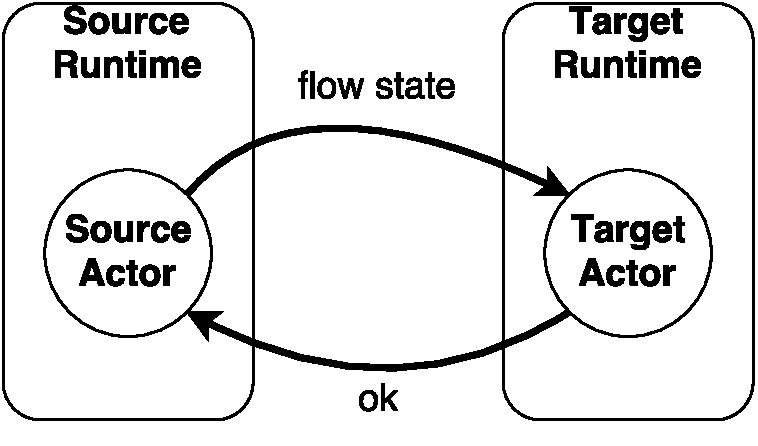
\includegraphics[width=\columnwidth]{figure/NFActor-Flow-Migration-Third.pdf}
		\caption{Migrate flow states}\label{fig:third}
	 \end{subfigure}
\caption{Distributed Flow Migration Protocol}
\label{fig:migration}
\end{figure*}

%The distributed flow migration protocol is shown in figure \ref{fig:migration}.
%It consists of passing 4 request-response. We first show successful
%request-response in figure \ref{fig:migration} and then supplement possible
%failure cases.

%As shown in figure \ref{fig:init}, the flow
%migration in NFActor is initiatied by sending a {\tt start\_migration} message
%from the NFActor runtime 1 to an actor \textit{a} on this runtime. The {\tt
%start\_migration} message contains a ID of a target runtime. Runtime 1 acquires
%this ID by querying the view service. Once actor \textit{a} receives this
%message, it starts the migration process by itself, without involving a centralized controller.
%Runtime 1 is promised to receive a response from actor \textit{a}. A {\tt
%migration\_ok} message sent from actor \textit{a} indicates that the migration
%is successfully finished. The flow being migrated has
%resumed its execution on the target runtime. Actor \textit{a} has quit
%execution and released all its resources. The migration can of course fail due
%to many reasons. In that case, actor \textit{a} will respond a {\tt
%migration\_fail} message back to runtime 1 and continue to process flow packets
%on runtime 1.

%The over-all workflow of the distributed flow migration protocol is illustrated in figure \ref{fig:migration}. The migration involves migrating a source actor from the source runtime to a target actor on the target runtime. We first discuss successful flow migration procedure, then we supplement possible failures that may interrupt the flow migration procedure.

\textbf{Create Target Actor (Fig.~\ref{fig:first})}: The source actor %(\chuan{should it be source actor instead since you just said the actor handles the migration all by itself}) 
sends a `create target actor' message to the target runtime. This message also contains the flow identifier of the actor handling the flow to be migrated (\ie, source actor). Upon receiving the message, the target runtime creates a target actor, configures the NF modules, and registers the target actor with the flow identifier, so that the target actor can correctly receive forwarded packets of the flow from the virtual switch. The target runtime sends an `ok' message back to the source actor.

\textbf{Contact Virtual Switch (Fig.~\ref{fig:second})}: After finishing the first pass of request-response, the source actor then sends a `forward to target runtime' message to the virtual switch, carrying the flow identifier of the source actor and the ID of the target runtime. After receiving this message, the virtual switch updates its switching hash table by changing the MAC address associated with the flow 5-tuple %\chuan{the hash table maps the flow 5-tuple to mac address, so is the flow identifier the 5 tuple? Unify the descriptions} 
to the MAC address of the target runtime. Then the virtual switch sends an `ok' message back to the source actor. Instead of being a control plane message, this `ok' message is carried in a data plane packet with the same flow identifier (that the source actor is handling), whose content is a global unique magic number %\chuan{shouldn't the content be just `ok'? what is this magic number used for?}
. We use a unique magic number to prevent the content of the flow packet from interfering the migration protocol. When the source actor receives this data plane response packet, it knows that there are no more data-plane packets of the flow coming to it and it can safely proceed to the final pass of request-response. The use of a data plane response packet ensures lossless flow migration \cite{gember2015opennf} without incurring more message passing overhead %\chuan{discuss the main idea why using data plan response can ensure lossless flow migration}
. The data plane response is sent after the virtual switch updates its hash table. Because data plane packet comes in order (re-order may happen, but rarely), whenever the migration source actor receives the data plane response, it can ensure that it will not receive any more data plane packets so that it can safely continue without missing any data plane packet. 

After the hash table update at the virtual switch, the packets of the flow are now forwarded to the target runtime, which dispatches them to the target actor. The target actor buffers the received flow packets without actually processing it, until the flow migration is completed.



\textbf{Migrate Flow States (Fig.~\ref{fig:third})}: The source actor serializes all the flow states using the API provided by each NF module (Fig.~\ref{fig:api}). Then the source actor sends the serialized flow states to the target actor. After receiving the serialized flow states, the target actor immediately sends back an `ok' message to indicate migration success. Then it processes all the buffered packets and resumes normal flow packet processing. After receiving the `ok' message from the target actor, the source actor notifies the source runtime about the successful migration, performs cleanups and quits.



%Actor \textit{a} then sends a {\tt create\_target\_actor} request message to the
%target runtime 2, expecting a response. This message also contains the flow
%identifier of actor \textit{a}. Target runtime 2 target runtime 2 creates a target
%actor \textit{b}, registers target actor \textit{b} using the flow identifer
%contained in the {\tt start\_migration} message and delegates the migration
%process to target actor \textit{b}. Target actor \textit{b} then responds a {\tt
%ok} message to actor \textit{a}.

%\textbf{Contact Virtual Switch:} Actor \textit{a} sends a {\tt
%forward\_to\_target\_runtime} request message to the virtual switch. This
%message contains the flow identifier and the ID of the target runtime 2. After
%virtual switch has received the request message, the virtual switch first
%updates its switching hash table by changing the value associated with the flow identifier
%to the ID of target runtime 2. Then the virtual switch creates a data-plane
%packet with the same flow identifier contained in the message and fills the
%payload with a global unique magic-number. Then the virtual switch sends this
%data-plane packet back to runtime 1.

%When actor \textit{a} receives the data-plane packet with the magic number, it
%knows that the no more flow packets will be forwarded to itself. Then actor
%\textit{a} can safely migrate its flow state to the target actor \textit{b}. The
%use of the data-plane packet instead of control message ensures lossless flow
%migration \cite{gember2015opennf}. In case that actor \textit{a} fails to
%receive data-plane response packet after a timeout, actor \textit{a} will
%re-send {\tt forward\_to\_target\_runtime} to the virtual switch.

%After virtual switch updates its switching hash table, target actor \textit{b}
%starts to receive flow packets. Target actor \textit{b} only buffers these
%packets and waits until flow state migration complete before processing them.

%\textbf{Migrate Flow State:} Actor \textit{a} sends a {\tt migrate\_flow\_state}
%request message, along with the serialized flow states of actor \textit{a}, to
%target actor \textit{b}. After receving the request message, target actor
%\textit{b} first responds a {\tt ok} message back to actor \textit{a}.
%Then it drains all the buffered packets and resumes normal flow packet
%processing. 

%Actor \textit{a} on the other hand, waits until it receives {\tt ok} message
%from target actor \textit{b}. Then it responds a {\tt migration\_ok} message
%back to runtime 1, destroies all the of its resources and quits.

\subsection{Controlling the Maximum Number of Concurrent Migrations}

The runtime controls the maximum number of concurrent migrations that is allowed to perform in the system. This is because too many concurrent migrations may quickly overloads the migration target runtime as the traffic is now rescheduled to the migration target runtime. The runtime thus closely monitors the number of concurrent migrations. If the number surpasses a threshold, the runtime stops any further migrations. 

\subsection{Failure Handling}
 
Failures may happen during the execution of the above flow migration steps. Before the source actor receives the final acknowledgement from the target actor in the last step (Fig.~\ref{fig:third}), any failure will terminate the migration process and flow processing on the source actor should be properly resumed. We next discuss how the flow migration protocol handles failure.
 
\textbf{Messages lost in the network.} In each of the three steps (Fig.~\ref{fig:first} to \ref{fig:third}), if either
the request message or the response message is lost, the source actor will be interrupted by a timeout and will terminate its flow migration process. This further leads to a timeout on the target actor, which will terminate the target actor. Step 2 (Fig.~\ref{fig:second}) and step 3 (Fig.~\ref{fig:third}) involve changing packet forwarding path and migrating flow states. Therefore, before terminating the migration process, the source actor also sends a request to the virtual switch to change the forwarding path back to itself.

\textbf{Runtime failure or virtual switch failure.} During the migration process, the source (target) runtime keeps monitoring the liveness of the target (source) runtime and the virtual switch. %If a failure occurs, the source (target) actor receives a notification message sent from the runtime system. 
In case that the target runtime or the virtual switch fails, the source actor receives a notification from its runtime, immediately terminates the migration process and sends a request to the virtual switch (after its recovery if it fails) to change the forwarding path back to itself. In case that the source runtime fails, the target actor sends the request to the virtual switch to change the forwarding path back to the source actor (which will be recovered by the fault tolerance mechanism). Since the migration process is not logged, after the source runtime and the source actor are recovered, the source actor resumes processing the flow without knowing its previous migration attempt. 

In any case of a migration failure, the source runtime will select another migration target runtime for the flow, and run the flow migration protocol again.

%In figure \ref{fig:first}, the failure of either runtime
%simply halts the migration process. In figure \ref{fig:second} and
%\ref{fig:third}, actor \textit{a} and target actor \textit{b} monitor each
%other. The failure of runtime 1 causes target actor \textit{b} not to receive
%{\tt migrate\_flow\_state} message. Actor \textit{b} requests the virtual switch
%to forward to runtime 1. The failure of target runtime 2 causes actor \textit{a}
%to perform a live recovery. 

%\textbf{Buffer Overloads.} After virtual switch updates its switching hash
%table, target actor \textit{b} starts to buffer the packets. We set a maximum
%capacity for the buffer. If the buffer is full when receiving {\tt
%migrate\_flow\_state} message, target actor \textit{b} responds a {\tt fail}
%message to actor \textit{a}, causing \textit{a} to perform a live recovery.

%\textbf{Virtual Switch Fails.} After virtual switch is restarted, it may lost
%some states in the switching hash table. The flow being migrated may be forced
%to terminate due to inconsistent state.






